\documentclass[a4paper,10pt]{scrartcl}

% Inclusión de paquetes
\usepackage[utf8]{inputenc}
\usepackage{amsmath}
\usepackage{amssymb}
\usepackage{enumerate}
\usepackage{verbatim}
\usepackage{amsthm}
% Imágenes
\usepackage{graphicx}
\usepackage{tikz}
\usetikzlibrary{arrows}

% Definiciones
\theoremstyle{definition}
\newtheorem*{mydef}{Definición}
%\newtheorem{mydefn}{Definición}
\newtheorem*{theorem}{Teorema}
\newtheorem*{fact}{Proposición}
\newtheorem*{corollary}{Corolario}
\newtheorem*{eg}{Ejemplo}
\everymath{\displaystyle} % Displaystyle por defecto

% Comandos
\newcommand{\Referencia}[4]{\indent #1, \textbf{#2}. \textit{#3}, \textit{#4}.\\}
\renewcommand\refname{Referencias}
\renewcommand\contentsname{Contenidos}
\numberwithin{equation}{section}
\setlength{\parindent}{0cm} % Sin sangrías
\setlength{\parskip}{0.1cm}

% Sintaxis: \Algoritmo{Elementos de entrada}{Elementos de proceso}{Elementos de salida}
\newcommand{\Algoritmo}[3]{\textbf{Entrada} \begin{itemize} #1 \end{itemize} \textbf{Proceso} \begin{enumerate} #2 \end{enumerate} \textbf{Salida} \begin{itemize} #3 \end{itemize}}

\title{Teoría de Colas}
\author{
  Marta Andrés\and
  Ignacio Cordón\and
  Bartolomé Ortiz\and
}
\date{}

\begin{document}
\maketitle

\begin{center}
	
\includegraphics[width=0.4\textwidth]{./imgs/by-nc-sa.png}
\end{center}

\tableofcontents
\pagebreak

\section{Preliminares}

\subsection{Distribución exponencial}

Una variable aleatoria continua $X$ tiene distribución exponencial de parámetro $\lambda > 0$ si su función de distribución
$F$ viene dada por:

\[F(x) = \left\{\begin{array}{ll}
         1- e^{-\lambda x} ,& x\ge 0\\
         0 ,& x\le 0
         \end{array}\right.\]
         
Lo notamos $X \sim exp(\lambda)$

\subsubsection{Propiedad de Markov de la distribución exponencial}

\begin{mydef}
 Decimos que una variable aleatoria $X$ tiene la propiedad de Markov (o que no tiene memoria) si se verifica:
 \[P[X \le t+s \mid X \ge t] = P[0\le X \le s] \qquad \forall t,s \in \mathbb{R}, s\ge 0\]
\end{mydef}

Es decir, la probabilidad de que la variable aleatoria tome un valor en un intervalo no depende del intervalo en sí,
sino solo de la longitud del intervalo.

%% ¿Qué es exactamente la propiedad de Markov?
\begin{fact}
 Sea $X$ variable aleatoria tal que: $X \sim exp(\lambda)$. Entonces $X$ tiene la propiedad de Markov, esto es:
 
 \[P[X \le t+s \mid X \ge t] = P[0\le X \le s] \]
\end{fact}

\begin{proof}
 \begin{align*}
 P[X \le t+s \mid X\ge t] & =  \frac{P[X\le t+s, X\ge t]}{P[X\ge t]} = \frac{e^{-\lambda t+s} - e^{-\lambda t}}{e^{-\lambda t}} = \\
                            & =  1 - e^{-\lambda s} = P[0\le X \le s]
 \end{align*}
\end{proof}



\begin{theorem}
 La distribución exponencial es la única distribución continua que cumple la propiedad de Markov
\end{theorem}

\begin{proof}
 Sea la variable aleatoria continua $X$ con función de distribución: \[F(t) = P[X\le t]\]
 
 Se tiene que cumplir por la propiedad de no memoria:
 
 \begin{align*}
   &P[X \le s + t \mid X > t] = P[X \le s] \Leftrightarrow \\
   &\Leftrightarrow 1 - P[X \le s + t \mid X > t] = 1 - P[X \le s] \Leftrightarrow\\
   &\Leftrightarrow P[X > s + t \mid X > t] = P[X > s] \Leftrightarrow \\
   &\Leftrightarrow \frac{P[X > s + t, X > t]} = P[X > t] P[X > s]
 \end{align*}
 
  Es decir, llamando $G(x) = P[X > x]$ hemos probado $G(t+s) = G(t) G(s)$ para todo $t\in \mathbb{R}, s > 0$
 
  Además se tiene claramente que $G$ es decreciente y no negativa.
  
  \[G(0 + 0) = G(0)G(0) \implies G(0) \in \{0,1\}\]
  
  Pero si $G(0) = 0$ entonces $G(t) = G(t+0) = G(t)G(0)$ para todo $t\in \mathbb{R}$, contradicción por tenerse $G = 1-F$ y $F$ una función de distribución.
  
  Luego $G(0) = 1$
  
  Además desde $1 = G(0) = G(-t + t) = G(-t) G(t)$ se tiene $G(-t) = G(t)^{-1}$ para $t > 0$ (nótese que como $G$ es decreciente, $G(-t) > G(0) = 1$). De aquí se deduce también
  que $G$ es estrictamente positiva.
  
  Por inducción se puede probar fácilmente:
  
  \[G(nt) = G((n-1)t) G(t) = \ldots = G(t)^{n}, \qquad \forall t\in \mathbb{R}, n\in \mathbb{N}\]

  En particular, $G(n) = G(1)^n$ para cualquier $n\in \mathbb{N}$.
  
  Por último dados $p,q \in \mathbb{N}$:
  
  \[G\left(\frac{p}{q}\right)^q = G\left(\frac{p}{q} q\right) = G(1)^p \implies G\left(\frac{p}{q}\right) = G(1)^{\frac{p}{q}}\]
  
  Luego como $F$ es continua, $G$ lo es, y para cada $x \in \mathbb{R}$ podemos tomar $\{r_n\} \rightarrow x$ sucesión de racionales,
  y se tiene:
  
  \[G(x) = G(1)^x = e^{ln(G(1)) x}\]
  
\end{proof}


\subsection{Procesos de Poisson}

\subsubsection{Notación O pequeña}
  \begin{mydef} 
  Una función $f$ se dice $o(h)$ (formalmente $o\in o(h)$) y lo notamos $f=o(h)$ si se verifica:
  
  \[\lim_{h\rightarrow 0} \frac{f(h)}{h} = 0\]
  \end{mydef}

  Es decir, una función $f(h)$ es $o(h)$ si al compararla con $h$ suficientemente pequeño, podemos despreciar su
  valor.

  \begin{fact}
  Dados $c_1, \ldots c_n \in \mathbb{R}$, $f_1, \ldots f_n \in o(h)$, entonces $\sum_{i=1} c_i f_i = o(h)$
  \end{fact}

  \begin{proof}
  \[\lim_{h\rightarrow 0} \frac{\sum_{i=1} c_i f_i}{h} = \sum_{i=1}^n{c_i \lim_{h\rightarrow 0} \frac{f_i}{h}} = 0\]
  \end{proof}

\subsubsection{Proceso de Poisson}

  \begin{mydef} \textbf{Proceso de conteo}\\
  $\{N_t\}_{t\ge 0}$, proceso estocástico discreto, es proceso de conteo si se verifica:
  \begin{enumerate}
    \item No negatividad: $N_t \in \mathbb{N}\cup\{0\}, \quad \forall t\ge 0$. Además: $N(0)=0$
    \item Monotonía: $N_s \le N_t, \quad s \le t$
  \end{enumerate}

  $N_t$ indica el número de eventos que han ocurrido en el intervalo $[0,t]$. Por tanto $N_t- N_s$, con $t\ge s$
  indica el número de eventos que han ocurrido en $]s,t]$.
  \end{mydef}


  \begin{mydef} \textbf{Proceso de Poisson}\\
  Un proceso de conteo $\{N_t\}_{t\ge 0}$ verifica que es de Poisson de parámetro $\lambda > 0$ si se verifica:
  
  \begin{enumerate}
    \item El proceso tiene incrementos independientes: dados $0 \le t_1 < \ldots < t_n$, se verifica que
    las variables $N_{t_0}, N_{t_1} - N_{t_0}, \ldots N_{t_n}- N_{t_{n-1}}$ son independientes. Esto es, el número de eventos
    que se producen en intervalos disjuntos es independiente.
    \item El proceso tiene incrementos estacionarios: $N_{t+h}, N_t$ tienen la misma distribución para cualesquiera
    $t\ge 0, h\ge 0$
    \item $P[N_h = 1] = \lambda h + o(h)$, es decir, la probabilidad de que ocurra un evento en un intervalo de
    tiempo de longitud $h$ es casi proporcional a $h$, salvo por un término despreciable en comparación con dicho $h$, para
    $h$ suficientemente pequeño.
    \item $P[N(h) \ge 2] = o(h)$
  \end{enumerate}

  Se deduce que: 
  \[P[N_h = 0] = 1 - P[N_h=1] - P[N(h) \ge 2] = 1 -\lambda h - o(h)\]
  \end{mydef}


La mayoría de modelos de colas asumen una distribución exponencial para tiempos entre llegadas y tiempos 
de servicio, o equivalentemente una distribución de Poisson para frecuencias de llegada y servicio.

\begin{theorem}
 Sea $\{N_t\}_{t\ge 0}$ un proceso de Poisson de parámetro $\lambda > 0$. Entonces la variable aleatoria $Y$ que
 describe el número de eventos en cualquier intervalo de longitud $t > 0$ tiene una distribución de Poisson de parámetro
 $\lambda t$
 
 \[P[Y = k] = P[N_t = n] = e^{-\lambda t} \frac{(\lambda t)^k}{k!}, \quad k\ge 0\]
 
 %% Prueba: falta por hacer.
\end{theorem}


\begin{theorem}
 Sea $\{N_t\}_{t\ge 0}$ proceso de conteo. Sean $0 < t_n$ con $t_{n} < t_{n+1}, \quad \forall n\in 
 \mathbb{N}$ tiempos de eventos con $\tau_1= t_1, \tau_{n+1} = t_{n+1} - t_{n}, \quad \forall n\in
 \mathbb{N}$ tiempos entre llegadas. Entonces equivalen:
 
 \begin{itemize}
  \item $\{N_t\}_{t\ge 0}$ es proceso de Poisson
  \item Los tiempos entre llegadas $\{\tau_n\}$ son variables exponenciales i.i.d. de media $\frac{1}{\lambda}$
 \end{itemize}

\end{theorem}

%% Prueba: falta por hacer.

\begin{theorem}
 Sea $\{N_t\}_{t\ge 0}$ proceso de Poisson donde un evento ha tenido lugar en $[0,t]$. Entonces siendo $Y$ la variable
 describiendo el número de eventos en cualquier intervalo de longitud $t > 0$, entonces $Y \sim U([0,t])$.
\end{theorem}

%% Prueba: falta por hacer.

\subsection{Procesos de nacimiento y muerte}

El parámetro $\lambda$ de un proceso de Poisson $\{N_t\}_{t\ge 0}$ puede ser visto como una tasa de nacimiento, ya que la probabilidad
de que ocurra un evento en un intervalo de longitud $h$ es $P[N(h)-N(0)=1] = \lambda h e^{-\lambda h} = \lambda h + o(h)$.
Cuando suponemos que el parámetro no es constante, sino que depende de $n$ (cantidad de eventos que se han producido hasta el momento), esto
es $\lambda_n$, entonces la cantidad de nacimientos (eventos producidos) en un intervalo de longitud $h$ es $\lambda_n h + o(h)$. Si además
establecemos que se pueden producir muertes con una tasa $\mu_n$, donde la probabilidad de que se produzca una muerte en un intervalo de longitud
$h$ es $\mu_n h + o(h)$ tenemos un proceso de nacimiento y muerte.

\begin{mydef}
 Sea una cadena de Markov $\{N_t\}_{t\ge 0}$ con espacio de estados $\mathbb{N}\cup \{0\}$, donde el espacio de estados representa el número de individuos
 de un sistema (población). Entonces $\{N_t\}_{t\ge 0}$ se dice proceso de nacimiento y muerte si existen tasas no negativas de nacimiento y muerte,
 $\{\lambda_n\}_{\mathbb{N}\cup \{0\}}$ y $\{\mu_n\}_{\mathbb{N}\cup \{0\}}$ y se verifica:
 
 \begin{enumerate}
  \item La población puede aumentar o decrecer únicamente de uno en uno.
  \item Si el sistema está en estado $n\ge 0$ entonces el tiempo hasta que el sistema está en estado $n+1 \ge 0$ es una variable aleatoria exponencial
  de paŕámetro $\lambda_n$
  \item Si el sistema está en estado $n\ge 1$ entonces el tiempo hasta que el sistema está en estado $n-1 \ge 0$ es una variable aleatoria exponencial
  de paŕámetro $\mu_n$
 \end{enumerate}
\end{mydef}

Llamando $P_n(t) = P[N_t = n]$ se verifica:

Sea $h>0$ suficientemte pequeño. Entonces la probalidad $P_n(t+h)$ viene dada por la suma de la probabilidad de 
los siguientes hechos disjuntos:

\begin{enumerate}
 \item En $t$ el sistema tenía población $n$ y no se han producido muertes ni nacimientos hasta $t+h$, esto es:
 
 \begin{align*}
  &P[N_{t} = n, \nexists t<s<t+h: N_{s} \neq n] =\\
  &= P[N_{t+h}=n] \cdot (1-\lambda_n h + o(h)) \cdot (1-\mu_n h + o(h))= \\
  &= P_n(t)[1+\mu_n h + o() -\lambda_n h + \lambda_n \mu_n h^2 - \lambda_n h o(h) + o(h)] = \\
  &= P_n(t)(1-\lambda_n h - \mu_n h) + o(h)
 \end{align*}
 
 Donde se ha usado independencia de nacimientos y muertes y agrupación de todas las funciones que son $o(h)$
 
 \item En $t$ el sistema tenía población $n-1$ y se ha producido un único nacimiento entre $t$ y $t+h$:
 
 \[P_{n-1}(t) (\lambda_{n-1}h + o(h)) = P_{n-1}(t) \lambda_{n-1} h + o(h)\]
 
 \item En $t$ el sistema tenía población $n+1$ y se ha producido una única muerte entre $t$ y $t+h$:
 
 \[P_{n+1}(t) (\mu_{n+1} h + o(h))\]
 
 \item La probabilidad de que ocurran 2 o más transiciones entre $t$ y $t+h$ es $o(h)$ por hipótesis
\end{enumerate}


Sumando y simplificando funciones $o(h)$:

\[P_n(t+h) = [1-\lambda_n h -\mu_n h] P_n(t) + \lambda_{n-1} h P_{n-1}(t) + \mu_{n+1} h P_{n+1}(t) + o(h)\]


que diviendo por $h$ en ambos términos y operando, da lugar a:

\[\frac{P_n(t+h) - P_n(t)}{h} = -(\lambda_n + \mu_n) P_n(t) + \lambda_{n-1} P_{n-1}(t) + \mu_{n+1}P_{n+1}(t) + \frac{o(h)}{h}\]

Tomando límite en $h\rightarrow 0$ llegamos a:

\begin{equation}
\frac{\partial P_n(t)}{\partial t} = -(\lambda_n + \mu_n) P_n(t) + \lambda_{n-1}P_{n-1}(t) + \mu_{n+1}P_{n+1}(t)
\label{eq:recp_n(t)}
\end{equation}

En el caso particuar $n=0$, tenemos $\mu_o = 0$ y $P_{-1}(t) = 0$. Por tanto:

\begin{equation}
 \frac{\partial P_0(t)}{\partial t} = -\lambda_0 P_0(t) \mu_{1}P_{1}(t)
 \label{eq:recp_0(t)}
\end{equation}


Supongamos en lo que sigue que existe la distribución límite, esto es 
$\lim_{t\rightarrow \infty}\{P_n(t)\} = p_n$ y haciendo $t\rightarrow \infty$ en \eqref{eq:recp_n(t)},
y en \eqref{eq:recp_0(t)} llegamos a que:

\begin{align*}
0 &= \lambda_{n-1} p_{n-1} + \mu_{n+1} p_{n+1} - (\lambda_n + \mu_n) p_n, \quad n\ge 1\\
0 &= \mu_1 p_1 -\lambda_0 p_0, \quad n=0
\end{align*}

Veamos por inducción que: $p_n = p_0 \prod_{i=1}^n \frac{\lambda_{i-1}}{\mu_i}, \quad n\ge 1$.

\begin{proof}
 Los casos $n=0, n=1$ cumplen trivialmente la recurrencia. Para $n>0$, aplicando hipótesis de inducción a $p_{n-1}, p_{n}$:
 
 \begin{align*}
 p_{n+1} &= \frac{\lambda_n + \mu_n}{\mu_{n+1}} p_n - \frac{\lambda_{n-1}}{\mu_{n+1}}p_{n-1} = \\
         &= \frac{\lambda_n + \mu_n}{\mu_{n+1}} p_0 \prod_{i=1}^n \frac{\lambda_{i-1}}{\mu_i} - 
            \frac{\lambda_{n-1}}{\mu_{n+1}} p_0 \prod_{i=1}^{n-1} \frac{\lambda_{i-1}}{\mu_i} = \\
         &= \frac{\lambda_n}{\mu_{n+1}} p_0 \prod_{i=1}^n \frac{\lambda_{i-1}}{\mu_i} + 
            \frac{\mu_n \lambda_{n-1}}{\mu_{n+1}\mu_n} p_0 \prod_{i=1}^{n-1} \frac{\lambda_{i-1}}{\mu_i} - 
            \frac{\lambda_{n-1}}{\mu_{n+1}} p_0 \prod_{i=1}^{n-1} \frac{\lambda_{i-1}}{\mu_i} = \\
         &= \frac{\lambda_n}{\mu_{n+1}} p_0 \prod_{i=1}^n \frac{\lambda_{i-1}}{\mu_i} = p_0 \prod_{i=1}^{n+1} \frac{\lambda_{i-1}}{\mu_i}
 \end{align*}
\end{proof}

Las probabilidades deben sumar $1$, esto es $1 = \sum_{n=0}^{\infty} p_n = p_0 \underbrace{\left(1 + \sum_{n=1}^{\infty} \prod_{i=1}^n \frac{\lambda_{i-1}}{\mu_i} \right)}_{S}$

Que la serie $S$ sea convergente es condición necesaria para que exista la distribución límite. 
De hecho, también es condición suficiente. Si dicha distribución existe se tendría: 

\begin{equation}
 p_0 = S^{-1} 
 \label{eq:relp0}
\end{equation}


\section{El modelo de un \textit{``sistema de encolado''}}
Un sistema de encolado es un sistema como el que se muestra en la figura \ref{fig:encolado}, en la que se consideran las siguientes variables aleatorias:

\begin{itemize}
\item [$c$]
  Número (fijo) de servidores o canales en el sistema, $c\in \mathbb{N} \cup \{+\infty\}$
\item [$\tau$]
  Variable aleatoria que describe el tiempo entre llegadas (de clientes).
\item [$S$]
  Variable aleatoria que describe el tiempo de servicio.
  %% o [que tarda un cliente en ser servido] ?
\item [$Q$]
  Variable aleatoria que describe el tiempo que espera un cliente en la cola.
  %% [incóginta?]
\item [$N_{S,t}$]
  Variable aleatoria que describe el número de clientes que están siendo servidos en el instante $t$.
  %% [dependerá de $\tau$, $s$, $c$? y de más cosas?]
\item [$N_{Q,t}$]
  Variable aleatoria que describe el número de clientes en la cola (esperando a ser servidos) en el instante $t$.
  %% [depende también?]
\end{itemize}

%% Imagen del modelo (hecho con tikz por si interesa para la presentación)
\begin{figure}
  \centering
  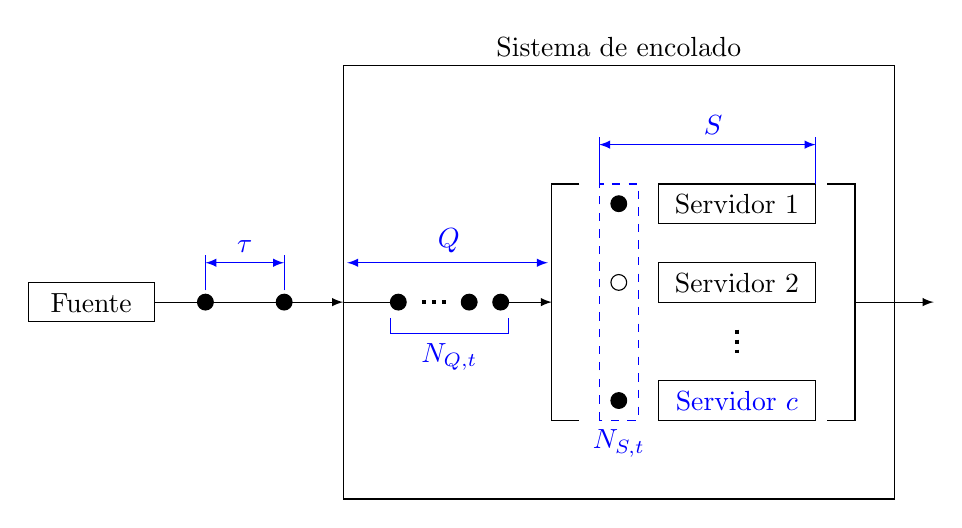
\begin{tikzpicture}
    \draw (20,5.5) rectangle (22,6);
    \node [above] at (21,5.5) {Servidor 1};
    \draw (20,4.5) rectangle (22,5);
    \node [above] at (21,4.5) {Servidor 2};
    \draw [dotted, ultra thick] (21,4.15) -- (21,3.85);
    \draw (20,3) rectangle (22,3.5);
    \node [above, blue] at (21,3) {Servidor $c$};

    \draw [fill] (19.5,5.75) circle [radius=0.1];
    \draw [fill=white] (19.5,4.75) circle [radius=0.1];
    \draw [fill] (19.5,3.25) circle [radius=0.1];
    \draw [dashed, blue] (19.25,3) rectangle (19.75,6);
    \node [below, blue] at (19.5,3) {$N_{S,t}$};

    \draw [latex-latex, blue] (19.25,6.5) -- (22,6.5);
    \draw [blue] (19.25,6) --(19.25,6.6);
    \draw [blue] (22,6) --(22,6.6);
    \node [above, blue] at (20.7,6.5) {$S$};

    \draw (22.15,6) -- (22.5,6) -- (22.5,3) -- (22.15,3);
    \draw [-latex] (22.5,4.5) -- (23.5,4.5);

    \draw (19,6) -- (18.65,6) -- (18.65,3) -- (19,3);
    \draw [-latex] (18,4.5) -- (18.65,4.5);
    \draw [fill] (18,4.5) circle [radius=0.1];
    \draw [fill] (17.6,4.5) circle [radius=0.1];
    \draw [dotted, ultra thick] (17,4.5) -- (17.3,4.5);
    \draw [fill] (16.7,4.5) circle [radius=0.1];
    \draw (16,4.5) -- (16.6,4.5);
    \draw [blue] (16.6,4.3) -- (16.6,4.1) -- (18.1,4.1) -- (18.1,4.3);
    \node [below, blue] at (17.35,4.1) {$N_{Q,t}$};

    \draw [latex-latex, blue] (16.05,5) -- (18.6,5);
    \node [above, blue] at (17.34,5) {$Q$};

    \draw (16,2) rectangle (23,7.5);
    \node [above] at (19.5,7.5) {Sistema de encolado};

    \draw (12,4.25) rectangle (13.6,4.75);
    \node [above] at (12.8,4.25) {Fuente};
    \draw [-latex] (13.6,4.5) -- (16,4.5);
    \draw [fill] (14.25,4.5) circle [radius=0.1];
    \draw [fill] (15.25,4.5) circle [radius=0.1];

    \draw [latex-latex, blue] (14.25,5) -- (15.25,5);
    \draw [blue] (14.25,4.65) --(14.25,5.1);
    \draw [blue] (15.25,4.65) --(15.25,5.1);
    \node [above, blue] at (14.75,5) {$\tau$};
  \end{tikzpicture}
  \caption{El modelo de un sistema de encolado.}
  \label{fig:encolado}
\end{figure}

%% Resaltar que $q$ no se conoce y es la que interesa conocer en general? $N_q[t]$ y $N_s[t]$ dependen también de otras cosas.

De ellos se derivan las siguientes variables, también relevantes:
\begin{itemize}
\item [$\lambda$]
  Frecuencia o tasa media de llegadas de clientes al sistema: $\lambda = 1/E[\tau]$.
\item [$\mu$]
  Frecuencia o tasa media de servicio de los servidores del sistema: $\mu = 1/E[S]$.
\item [$\rho$]
  Aprovechamiento de los servidores, esto es, la proporción de tiempo que los servidores están trabajando: $\rho = \frac{\lambda}{c\mu}$.
  %% $= \frac{E[N_s]}{c} = \frac{L_s}{c}$ por qué?
\item [$W_S$]
  Tiempo medio que está siendo servido un cliente: $W_S  = E[S]$.
\item [$W_Q$]
  Tiempo medio que está un cliente en la cola: $W_Q = E[Q]$.
\item [$W$]
  Variable aleatoria que describe el tiempo total que un cliente está en el sistema de encolado: $W = Q+S$.
\item [$W_W$]
  Tiempo medio que está un cliente en el sistema: $W_W = E[W]$.
\item [$N_S$]
  Variable aleatoria que describe el número de clientes siendo servidos con el sistema en equilibrio: $N_S = \lim_{t \rightarrow \infty} N_s[t]$.
\item [$L_S$]
  Número medio de clientes siendo servidos con el sistema en equilibrio: \\ $L_S = E[N_S]$.
\item [$N_Q$]
  Variable aleatoria que describe el número de clientes en la cola con el sistema en equilibrio: $N_Q = \lim_{t \rightarrow \infty} N_{Q,t}$.
\item [$L_Q$]
  Número medio de clientes en la cola con el sistema en equilibro: $L_Q = E[N_Q]$.
\item [$N_t$]
  Variable aleatoria que describe el número de clientes en el sistema en el instante $t$: $N_t = N_{Q,t} + N_{S,t}$.
\item [$N$]
  Variable aleatoria que describe el número de clientes en el sistema con el sistema en equilibrio (en caso de tener sentido) $N = N_Q + N_S$.
\item [$L$]
  Número medio de clientes en el sistema en equilibrio (en caso de tener sentido): $L = E[N]$.
\item [$P_n(t)$]
  Probabilidad de que haya $n$ clientes en el sistema en el instante $t$: es la función masa de probabilidad de $N_t$.
\item [$p_n$]
  Probabilidad de que haya $n$ clientes en el sistema con el sistema en equilibrio: $p_n = \lim_{t \rightarrow \infty} P_n(t)$ es la función masa de probabilidad de $N$.
\end{itemize}

\subsection{Características de un proceso de colas}
\subsubsection{Modelo de llegadas}
La capacidad de un sistema de colas para poder proporcionar servicio a los clientes no depende solo de la tasa media
de llegadas de un sistema de colas, sino también del modo en que las peticiones llegan. De esta forma, podemos
tener que las peticiones llegan de uno en uno, o en paquetes de peticiones.

Dado $0=t_0 < t_1 < t_2 < t_n < \ldots$, y $\tau_n = t_n - t_{n-1}, \tau_0$ tiempos entre llegadas, asumimos por hipótesis
que las $\tau_n$ son variables aleatorias independientes.

\begin{mydef}
LLamamos modelo de llegadas a la distribución de los $\{t_n\}$
\end{mydef}
 
 La distribución de los tiempos de llegada $\{t_n\}$ está determinada por la distribución de los tiempos entre
 llegadas $\{\tau_n\}$. 
 
\begin{mydef}
El modelo de llegadas se dice:
 
 \begin{enumerate}
   \item Estacionario, si las $\{\tau_n\}$ están idénticamente distribuidas, y notamos $\{\tau\}$ a la variable
   aleatoria que modela el tiempo entre llegadas.
   \item Transitorio, en caso opuesto.
 \end{enumerate}
\end{mydef}

 
\begin{mydef}
 Para un modelo de llegadas estacionario, sea $A(t)$ función de distribución de los $\tau_n$. 
 El modelo de llegadas se dice:

  \begin{enumerate}
  \item Aleatorio o de Poisson: si $A(t) = 1 - e^{-\lambda t}$
  \item Determinístico: si $A(t) = \left\{\begin{array}{ll}
					0 & t<s \\
					1 & t\ge s
					\end{array}\right.$ con $s$ fijo.
  
  \end{enumerate}
\end{mydef}


\subsubsection{Modelo de servicio}

Se pueden efectuar unas definiciones análogas para modelo determinístico, aleatorio y régimen estacionario y transitorio
de servicio a las que se han hecho con el modelo de llegadas.

\begin{eg} \textbf{Caso particular, modelo de Poisson de servicio}

Supongamos que el sistema de encolado tiene $k$ servidores o canales para atender peticiones, y el tiempo que 
tarda cada uno en atender una petición $T_i, i=1,\ldots k$ sigue una distribución exponencial de parámetro $\bar{\mu}$.
Entonces el tiempo hasta terminar de atender una petición es $T = min\{T_1, \ldots T_n\}$. Entonces $T$ sigue
una distribución exponencial de parámetro $\mu = n \bar{\mu}$

La función de distribución de $W_S$ por tanto sería $F(t) = P[S\le t] = 1 - e^{-\mu t}$
\end{eg}

\subsubsection{Capacidad del sistema}
Se llama capacidad al tamaño máximo de la cola de peticiones, esto es $M = \max_t \{N_{Q,t}\}$. Por tanto no puede
tenerse que en ningún tiempo $N_{Q,t}$ tome un valor mayor que $M$, y si llegara una petición cuando la cola tiene
tamaño $M$, se rechazaría dicha petición.

\subsubsection{Comportamiento de los clientes}
Podemos considerar que los clientes que llegan a la cola pueden efectuar:

\begin{itemize}
  \item Oposición: una petición se retira en la llegada (por ejemplo en casos en los que la cola sea muy larga
  y el cliente se abstenga de entrar).
  \item Retirada: la petición entra a la cola, pero tras un tiempo de espera, la deja.
  \item Recolocación: si hay varias colas paralelas, los clientes se pueden cambiar de una cola a otra.
  \item Priorización: algunos clientes pueden tener mayor prioridad que otros al ser servidos.
\end{itemize}

\subsubsection{Disciplina de la cola}
Se pueden tener distintas formas de elegir de la cola el siguiente cliente a ser servido. Consideramos las siguientes estrategias:
\begin{itemize}
\item FIFO (First in, first out): es la cola tradicional, en la que el cliente que lleva más tiempo esperando en la cola es el siguiente en ser servido.
\item LIFO (Last in, first out): el cliente que lleva menos tiempo esperando en la cola es el siguiente en ser servido.
\item SIRO (Service in random order): se escoge un cliente al azar de entre todos los de la cola, con probabilidad uniforme.
\item PRI (Priority  service): los clientes tienen asignado un nivel de prioridad y se elige el cliente con mayor prioridad de la cola. En caso de haber varios con la misma probabilidad, se usa alguna de las disciplinas anteriores para elegir entre ellos.
\end{itemize}

\subsection{Notación de Kendall}

Se utiliza para describir las características de una cola de forma breve la notación de Kendall, de la forma $A/B/c/K/m/Z$, donde:
\begin{itemize}
\item $A$ y $B$ describen $\tau$ (el tiempo entre llegadas) y $S$ (el tiempo de servicio) respectivamente, siendo los símbolos más comunes:
  \begin{itemize}
  \item [$G$]
    General, sólo se asume que $\tau_n$ o $S_n$ son independientes.
  \item [$D$]
    Determínistica, donde $\tau$ es constante.
  \item [$M$]
    De Markov, esto es, se usa la distribución exponencial para dar un proceso de llegadas llamado de Poisson o aleatorio.
  %% Estas dos no aparecen en en el apartado 2.1.1, ponerlas?
  %% \item [$E_k$] Erlang-k
  %% \item [$H_k$] k-stage hyperexponential
  \end{itemize}
\item $c$ describe el número de servidores, que puede ir desde 1 hasta infinito (aunque en teoría no se puede tener un número infinito de servidores, en la práctica se puede tener una cantidad de servidores suficientemente grande como para parecer infinita).
\item $K$ describe la capacidad máxima del sistema, esto es, el número máximo de clientes que puede haber en el sistema entre la cola y el servicio.
\item $m$ describe el tamaño de la población, que puede ir desde 1 hasta infinito.
\item $Z$ describe la disciplina de la cola, con las siglas usadas anteriormente (u otras equivalentes, mientras no haya ambigüedad).
\end{itemize}

A menudo, se asume que $K$ y $m$ son infinitos y $Z$ es de tipo FIFO, y se usa una notación acortada de la forma $A/B/c$.

\subsection{Medidas de efectividad}
Se pueden considerar disintos valores como medidas de efectividad del sistema, entre ellos, los siguientes:
\begin{itemize}
\item $\rho$:
  Aprovechamiento de los servidores, esto es, la proporción de tiempo que los servidores están trabajando: $\rho = \frac{\lambda}{c\mu}$. Cuanto más alta mayor es la eficiencia de los servidores, pero si $\rho > 1$ significa que el sistema está sobrecargado y aumentará el número de clientes en la cola, ya que entran clientes al sistema más rápido que salen.
\item $W_W$:
  Tiempo medio de un cliente en el sistema. Naturalmente, se desea minimizar el tiempo que tarda un cliente en ser servido.
\item $W_Q$:
  Tiempo medio de un cliente en la cola. Similar al anterior, pero en algunos casos puede interesar más el tiempo de espera en la cola solamente. Por ejemplo, en el caso de la cola en un supermercado, un cliente estará insatisfecho si tiene que esperar mucho tiempo en la cola, pero mientras está siendo servido está ocupado y no lo percibe como tiempo de espera.
\item $\pi_{W_W} \lbrack 90 \rbrack$:
  Percentil 90 de el tiempo total en el sistema $W_W$. En lugar de usar la media que puede ser afectada por casos extremos, se utiliza el tiempo de espera de una gran parte de los clientes, pudiendo variar el percentil que se considera según se desee.
\item $\pi_{W_Q} \lbrack 90 \rbrack$:
  Percentil 90 de el tiempo de espera en la cola $W_Q$. Análogamente al anterior, pero una vez más teniendo en cuenta únicamente el tiempo de espera en la cola y no el total.
\item $L$:
  Número medio de clientes en el sistema. En general, cuantos más clientes haya en el sistema mayor será su tiempo de espera. Sin embargo, si hay muchos servidores no necesariamente se puede optimizar el sistema, por tanto mientras $L<c$ no necesariamente es ineficiente el sistema.
\item [$L_Q$]
  Número medio de clientes en la cola. Como se explica en el punto anterior, el número medio de clientes en el sistema no necesariamente es representativo, y puede ser más útil considerar el número medio de clientes esperando en la cola, excluyendo así los que están siendo servidos.
\item [$p_n$]
  Probabilidad de que haya $n$ clientes en el sistema (en el estado de equilibrio). En general, interesa conocer su función de distribución para que la probabilidad de que haya $n$ o menos clientes en el sistema sea lo más alta posible para un $n$ adecuadamente pequeño.
\end{itemize}
\subsection{Leyes de Little}
Brevemente recordamos los conceptos ya nombrado anteriormente, pues será de ayuda tenerlos a mano durante la definición de los elementos que conforman el teorema.
Para $i \geq 1$, llamemos al cliente $c_i$, el cual llega en el instante $t_i$, nombremos $W_i$ al tiempo de espera del cliente con lo cual es inmediato deducir, que nuestro cliente abandonará la cola en el instante $t_i + W_i$, donde $t_0 \equiv 0 \leq t_1 \leq t_2 \leq... $.
Es inmediato tambien que podemos definir una funcion indicadora que refleje si el $c_i$ está o no en el sistema:

Indicador: $I_i(t) = 1 $ si $ t_i \leq t <t_i+W_i$,y $I_i (t) = 0$ en caso contrario,de donde  $\int_{0}^{\infty} I_i(t)dt=W_i$.

Sea $N(t) = \sum_{i=1}^{\infty} I_i(t)$, el número de clientes en el sistema en tiempo t, y $\Delta (t) = max \{i: t_i \leq t\}$, el número de llegadas en tiempo t. Con $\Delta (t)$, reescribimos $N(t) = \sum_{i=1}^{\Delta (t)} I_i(t)$.

De los datos del cliente ${t i}$ y ${W i}$ para todo i, podemos construir ${N (t)}$ para
todo t. Visualmente podemos entender de forma sencilla estos conceptos si trazamos ${\Delta (t)}$ como una función escalonada y mostramos un tiempo de espera del cliente.
\begin{center}
	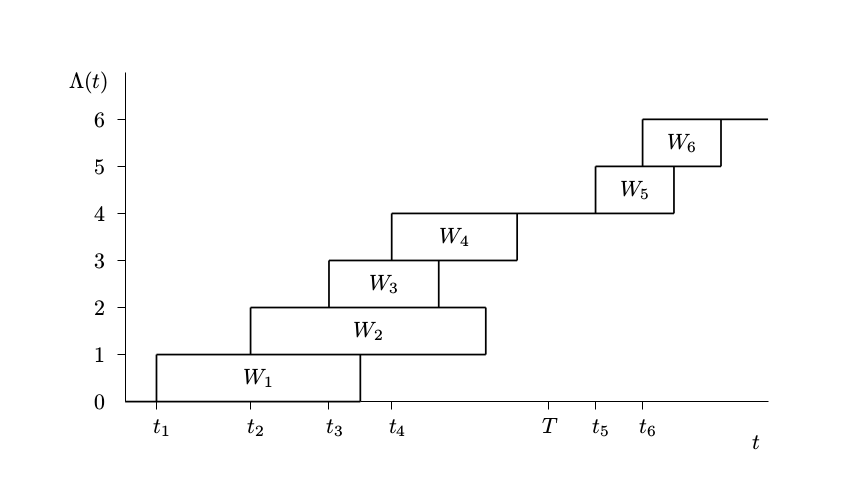
\includegraphics[width=\textwidth]{./imgs/fig1.png}
\end{center}
 A su vez podemos representar $N(t)$ como una función escalonada ( cuya información será obviamente menor que la primera figura) representando unicamente el numero de personas en la cola.
\begin{center}
	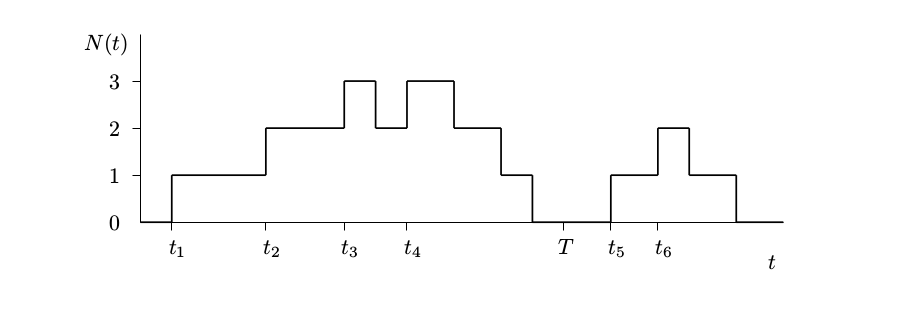
\includegraphics[width=\textwidth]{./imgs/fig2.png}
\end{center}

Mientras que los tiempos de espera son periodos de tiempo, también se pueden observar como rectángulos de altura 1 en la gráfica de ${\Delta(t)}$. Así, la longitud $W_i$ es también área $W_i$. Para cada t, $N (t)$ es simplemente el número de rectángulos de tiempo de espera que contienen el punto t.

Tenemos por tanto un modelo de colas (estocástico), con $ t_i, W_i $y$ N(t)$ variables aleatorias; lo que nos lleva trivialmente a asumir que  $\{T i, i \geq 1\}$, $\{W i, i \geq 1\}$, y $\{N (t), t \geq 0\}$ son procesos estocásticos. Estas cantidades aleatorias se definiran en un espacio muestral cualquiera. 

Por lo general, en nuestro caso se suelen hacer las siguientes suposiciones :
\begin{itemize}
	\item $W_i$ tiene la misma distribución para todo i.
	\item $N (t)$ tiene la misma distribución para todo t. 
\end{itemize} 

Llegados a este punto hemos de remarcar que existen realmente dos versiones de la Ley de Little: \begin{itemize}
	\item La versión que relaciona el tiempo de espera medio y la cantidad media de clientes en la cola: la mas conocida y a que trataremos en el trabajo.
	\item La versión estacionaria que relaciona los valores esperados de W y N través de la esperanza. 
\end{itemize}

Damos a continuación una idea intuitiva del primer teorema, que pensamos puede ayudar enormemente a nuestros compañeros (entre los cuales nos incluimos) a captar la esencia del resultado:

Nota: De ahora en adelante omitiremos el punto del espacio muestral en el que estamos. Esto no afecta en absoluto a nuestro trabajo y simplifica la notacion al no tener que acarrerar la dependencia explícita del mismo: Por ejemplo, escribimos $W_i$ en lugar de $W_i (\omega)$.

El área rectangular $W_i$ es la contribución al área bajo ${N (t)}$ que es realizada por el cliente $c_i$. Ahora considerese el área bajo ${N (t)}$ en algún intervalo$(0, T)$, donde como en las figuras 1 y 2, T tiene la propiedad de que $N (T) = 0$. Para cualquier T de esa forma, esta área puede escribirse como una integral o una suma,\[\int_{0}^{T} N(t)dt=\int_{0}^{T} \sum_{i=1}^{\Delta (t)} I_i(t) dt=(permtuando)=\sum_{i=1}^{\Delta (t)} W_i(t)  \]

Se puede observar en nuestras figuras en $\Delta(T) = 4$.

Para cualquier T donde $N (T)> 0$, (1) no es cierto porque una porción de al menos un rectángulo en la suma contribuye al área bajo $\{N (t)\}$ después de T. En este caso, la suma - integral $\equiv$ error $\geq 0$.

Entonces definimos la media de estas cantidades a largo plazo como límites, cuando existan, denominándolos como siguen
\begin{itemize}
	\item $L=\lim_{T\to\infty}\frac{1}{T}\int_{0}^{T} N(t)dt$
	\item $\omega=\lim_{n\to\infty}\frac{1}{n}\sum_{i=1}^{n} W_i(t)$
	\item $\lambda=\lim_{t\to\infty}\frac{\delta(t)}{t}$
\end{itemize}

Donde conceptualmente estamos haciendo referencia a:
\begin{itemize}
	\item $L$ es el número medio de clientes en el sistema,
	\item $\omega$ es el tiempo medio de espera (de los clientes en el sistema), y
	\item $\lambda$ es la tasa de llegada 
\end{itemize}
Es de destacar que  $L$ y $\omega$ son las dos medidas de rendimiento más comunes para una cola.


Tenemos ya todos los elementos para formular el teorema de Little:
\begin{theorem}{Teorema de Little}
Si los límites $\lambda$ y $\omega$ existen y son finitos, $L$ existe y es finito, donde
\begin{equation}
L = \lambda\omega
\end{equation} 
\end{theorem}

La idea intuitiva de este resultado es la relación que apúntabamos antes: Para cualquier T (donde ahora $N (T) \geq 0$) escribimos,
\[ \frac{\int_{0}^{T} N(t)dt}{T}=\frac{\sum_{i=1}^{\Delta (t)} W_i(t)}{T}-\frac{error}{T}=\frac{\Delta(T)}{T}\frac{\sum_{i=1}^{\Delta (T)} W_i(t)}{\Delta(T)}-\frac{error}{T}   \]
A medida que T se hace grande, la primera cantidad entre paréntesis a la derecha se aproxima a $\lambda$, la segunda a $\omega$, y el producto se acerca $\lambda\omega$. Por lo tanto, el teorema se obtendría si el término a la derecha se aproxima a 0 cuando $T\rightarrow\infty$. El término de error no tendría porqué hacerse pequeño, sólo crecer más lentamente que T.
Teniendo esta idea en mente, podemos proceder a demostrar el resultado formalmente:
\begin{proof}
Motivados por las Figuras 1 y 2, obtenemos las siguientes desigualdades en
\begin{equation}
 \sum_{\{i:t_i+W_i\leq T\}}^{} W_i\leq\int_{0}^{T}N(t)dt\leq \sum_{i=1}^{\delta(T)} W_i
 \label{DesiLi}
 \end{equation}
donde la suma a la izquierda está por debajo de aquellos rectángulos de espera que han terminado en T.
Ahora dividimos la expresión por T y hacemos tender $T\rightarrow\infty$. La expresión de la derecha tiene límite $\lambda\omega$,lo que implica que la integral tiene $lim sup \leq \lambda\omega$.Si conseguimos demostrarlo para el inferior concluiremos la demostración. Con ese fin, necesitamos dos resultados preliminares. Primero, escribimos:
\[ \frac{W_n}{n}=\frac{1}{n}\sum_{i=1}^{n}W_i-(\frac{n-1}{n})(\frac{1}{n-1})\sum_{i=1}^{n-1}W_i \]
Para $\omega$ finito, esta expresión tiene límite 0 si $n \rightarrow \infty$. Es decir,
\[ \lim_{n\to\infty} W_n / n = 0. \]

Si, ahora, $\lambda$ es finito, esto implica $t_n \rightarrow \infty$ y, $\delta(t_n)/t_n \rightarrow  \lambda$ como $n \rightarrow \infty$. Si los tiempos de llegada son distintos escribiriamos, $\delta(t_n)=n$; de lo contrario, $\delta(t_n)\geq n$, y escribimos:

\[ \frac{W_n }{t_n} = \frac{W_n }{n}\frac{n }{t_n}\leq \frac{W_n }{n}\frac{\delta(tn)}{t_n} \]
 tenemos por tanto:
 \[ \lim_{n\to\infty} W_n / t_n = 0. \]

Para cualquier $\epsilon> 0$, el anterior limite implica que para algún $m$ finito y todo $i> m$, $W_i <t_i\epsilon$ y $t_i + W_i <t_i (1 + \epsilon)$. Así, $t_i \leq T / (1 + \epsilon) \Longrightarrow t_i + W_i \leq T$ para cada $i> m$,lo que nos da esta cota inferior en la expresión de la izquierda en \ref{DesiLi} :
\begin{equation}\sum_{i=1}^{\delta(\frac{T}{1+\epsilon})} W_i-\sum_{i=1}^{m} W_i\leq \sum_{\{i:t_i+W_i\leq T\}}^{} W_i
\label{DesiLi2}
\end{equation}

Ahora dividimos por T y hacemos tender T a infinito, notando que el segundo término de la izquierda es un
constante. El lado izquierdo de \ref{DesiLi2} tiene límite $ \lambda\omega / (1 + \epsilon)$, lo que implica el lado derecho tiene lim inf $\geq \lambda\omega / (1 + \epsilon))$. Debido a que $\epsilon$ puede ser arbitrariamente pequeño, y combinando limite superior e inferior, concluimos la prueba.
\end{proof}

%% Ejemplo de cita: \cite{Ciarlet}

\newpage
\begin{thebibliography}{10}
  \expandafter\ifx\csname url\endcsname\relax
  \def\url#1{\texttt{#1}}\fi
  \expandafter\ifx\csname urlprefix\endcsname\relax\def\urlprefix{URL }\fi
  \expandafter\ifx\csname href\endcsname\relax
  \def\href#1#2{#2} \def\path#1{#1}\fi

\bibitem{Allen}
  Arnold O.Allen (1990)\\
  Probability, Statistics and Queueing Theory with Computer Science Applications\\
  Academic Press

\bibitem{Gross}
  Donald Gross, John F.Shortle, James M.Thompson, Carl M.Harris (2008)\\
  Fundamentals of Queueing Theory\\
  Wiley
  
\bibitem{Gunavathi}
  P.Kandasamy, K.Thilagavathi, K.Gunavathi\\
  Probability and Queueing Theory (2010)\\
  S. Chand \& Company

\bibitem{Ronald}
  Ronald W. Wolff\\
  Little's law and Related Results (2011)\\
  University of California at Berkeley
\end{thebibliography}

\end{document}
